% README file for moduleDocumentationTemplate TeX template.
% This template should be used to document all Basilisk modules.
% Updated 20170711 - S. Carnahan
%
%-Copy the contents of this folder to your own _Documentation folder
%
%-Rename the Basilisk-moduleDocumentationTemplate.tex appropriately
%
% All edits should be made in one of:
% sec_modelAssumptionsLimitations.tex
% sec_modelDescription.tex
% sec_modelFunctions.tex
% sec_revisionTable.tex
% sec_testDescription.tex
% sec_testParameters.tex
% sec_testResults.tex
% sec_user_guide.tex
%
%-Some rules about referencing within the document:
%1. If writing the suer guide, assume the module description is present
%2. If writing the validation section, assume the module features section is present
%3. Make no other assumptions about any sections being present. This allow for sections of the document to be used elsewhere without breaking.

%In order to import some of these sections into a document in a different directory:
%\usepackage{import}
%Then, the sections are called with \subimport{relative path}{file} in order to \input{file} using the right relative path.
%\import{full path}{file} can also be used if absolute paths are preferred over relative paths.

%%%%%%%%%%%%%%%%%%%%%%%%%%%%%%%%%%%%%%%%%%%%%%%%%




\documentclass[]{BasiliskReportMemo}

\usepackage{cite}
\usepackage{AVS}
\usepackage{float} %use [H] to keep tables where you put them
\usepackage{array} %easy control of text in tables
\usepackage{graphicx}
\bibliographystyle{plain}


\newcommand{\submiterInstitute}{Autonomous Vehicle Simulation (AVS) Laboratory,\\ University of Colorado}


\newcommand{\ModuleName}{Module Name}
\newcommand{\subject}{Module Name Model}
\newcommand{\status}{Status}
\newcommand{\preparer}{F. Last}
\newcommand{\summary}{Summary of the document goes here.}

\begin{document}

\makeCover

%
%	enter the revision documentation here
%	to add more lines, copy the table entry and the \hline, and paste after the current entry.
%
\pagestyle{empty}
{\renewcommand{\arraystretch}{2}
\noindent
\begin{longtable}{|p{0.5in}|p{3.5in}|p{1.07in}|p{0.9in}|}
\hline
{\bfseries Rev} & {\bfseries Change Description} & {\bfseries By}& {\bfseries Date} \\
\hline
1.0 & Revision Description & F. Last1 & YYYYMMDD\\
\hline
1.1 & Revision Description& F. Last2 & YYYYMMDD\\
\hline

\end{longtable}
}



\newpage
\setcounter{page}{1}
\pagestyle{fancy}

\tableofcontents %Autogenerate the table of contents
~\\ \hrule ~\\ %Makes the line under table of contents










	
\section{Model Description}

\subsection{Introduction}

The hinged rigid body class is an instantiation of the state effector abstract class. The state effector abstract class is a base class for modules that have dynamic states or degrees of freedom with respect to the rigid body hub. Examples of these would be reaction wheels, variable speed control moment gyroscopes, fuel slosh particles, etc. Since the state effectors are attached to the hub, the state effectors are directly affecting the hub as well as the hub is back affecting the state effectors.

Specifically, a hinged rigid body state effector is a rigid body that has a diagonal inertia with respect to its $\mathcal{S}_i$ frame as seen in Figure~\ref{fig:FlexFigure}. It is attached to the hub through a hinge with a linear torsional spring and linear damping term. The dynamics of this multi-body problem have been derived and can be seen in Reference~\cite{Allard2016rz}. The derivation is general for $N$ number of panels attached to the hub but does not allow for multiple interconnected panels. 

\begin{figure}[htbp]
	\centerline{
		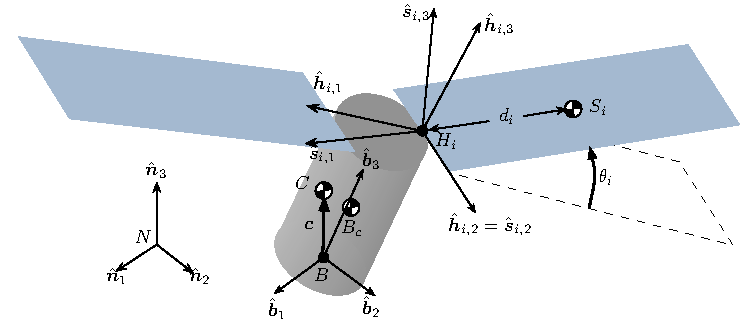
\includegraphics[width=0.8\textwidth]{Figures/Fig4_4_2}}
	\caption{Hinged rigid body frame and variable definitions}
	\label{fig:FlexFigure}
\end{figure}

\subsection{Equations of Motion}

The following equations of motion (EOMs) are pulled from Reference~\citenum{Allard2016rz} for convenience. Equation~\eqref{eq:Rbddot3} is the spacecraft translational EOM, Equation~\eqref{eq:Final6} is the spacecraft rotational EOM, and Equation~\eqref{eq:solar_panel_final3} is the hinged rigid body rotational EOM. These are the coupled nonlinear EOMs that need to be integrated in the simulation. 

\begin{multline}
m_{\text{sc}} \ddot{\bm r}_{B/N}-m_{\text{sc}} [\tilde{\bm{c}}]\dot{\bm\omega}_{\cal B/N}+\sum_{i}^{N}m_{\text{sp}_i} d_i  \bm{\hat{s}}_{i,3}\ddot{\theta}_i = \bm F_{\textnormal{ext}} - 2 m_{\text{sc}} [\tilde{\bm\omega}_{\cal B/N}]\bm{c}'\\
-m_{\text{sc}} [\tilde{\bm\omega}_{\cal B/N}][\tilde{\bm\omega}_{\cal B/N}]\bm{c}-\sum_{i}^{N}m_{\text{sp}_i}d_i\dot{\theta}_i^2 \bm{\hat{s}}_{i,1}
\label{eq:Rbddot3}
\end{multline}

\begin{multline}
	m_{\text{sc}}[\tilde{\bm{c}}]\ddot{\bm r}_{B/N}+[I_{\text{sc},B}] \dot{\bm\omega}_{\cal B/N} +\sum\limits_{i}^{N}\biggl\lbrace I_{s_i,2}\bm{\hat{h}}_{i,2}+m_{\text{sp}_i}d_i [\tilde{\bm{r}}_{S_i/B}] \bm{\hat{s}}_{i,3}\biggr\rbrace\ddot{\theta}_i = \\
	-[\bm{\tilde{\omega}}_{\cal B/N}] [I_{\text{sc},B}] \bm\omega_{\cal B/N} 
	- [I'_{\text{sc},B}] \bm\omega_{\cal B/N} - \sum\limits_{i}^{N}\biggl\lbrace\dot{\theta}_i [\bm{\tilde{\omega}}_{\cal B/N}] \left(I_{s_i,2} \bm{\hat{h}}_{i,2}+m_{\text{sp}_i} d_i [\tilde{\bm{r}}_{S_i/B}] \hat{\bm s}_{i,3}\right)\\ +m_{\text{sp}_i}d_i\dot{\theta}_i^2[\tilde{\bm{r}}_{S_i/B}] \bm{\hat{s}}_{i,1} \biggr\rbrace + \bm{L}_B
	\label{eq:Final6}
\end{multline}

\begin{multline}
m_{\text{sp}_i} d_i \hat{\bm s}_{i,3}^{T} \ddot{\bm r}_{B/N}+ \biggl[\left(I_{s_{i,2}} + m_{\text{sp}_i}d_i^{2}\right) \hat{\bm s}_{i,2}^{T}-m_{\text{sp}_i} d_i \hat{\bm s}_{i,3}^{T} [\tilde{\bm r}_{H_i/B}]\biggr] \dot{\bm\omega}_{\cal B/N} \\
+ \left( I_{s_{i,2}} + m_{\text{sp}_i} d_i^{2} \right) \ddot \theta_i 
= - k_i \theta_i - c_i \dot\theta_i + \hat{\bm s}_{i,2}^T \bm \tau_{\text{ext},H_i} + \left( I_{s_{i,3}} - I_{s_{i,1}} + m_{\text{sp}_i}d_i^{2}\right) \omega_{s_{i,3}} \omega_{s_{i,1}}\\
- m_{\text{sp}_i} d_i \hat{\bm s}_{i,3}^{T} [\tilde{\bm\omega}_{\cal B/N}][\tilde{\bm\omega}_{\cal B/N}] \bm r_{H_i/B} 
\label{eq:solar_panel_final3}
\end{multline}

\subsection{Back Substitution Method}

In order to integrate the EOMs in a modular fashion, a back substitution method was developed and can be seen in Reference~\cite{Allard2016rz}. The hinged rigid body model must adhere to this analytical form, and the details are briefly summarized in the equations following. First the hinged rigid body EOM is substituted into the translational EOM and rearranged:
\begin{multline}
\Big(m_{\text{sc}} [I_{3\times3}] +\sum_{i=1}^{N}m_{\text{sp}_i}d_i \bm{\hat{s}}_{i,3} \bm a_{\theta_i}^T\Big)\ddot{\bm r}_{B/N}+\Big(-m_{\text{sc}} [\tilde{\bm{c}}] +\sum_{i=1}^{N}m_{\text{sp}_i}d_i \bm{\hat{s}}_{i,3} \bm b_{\theta_i}^T\Big) \dot{\bm\omega}_{\cal B/N} \\
= m_{\text{sc}} \ddot{\bm r}_{C/N} 	- 2 m_{\text{sc}} [\tilde{\bm\omega}_{\cal B/N}] \bm c'
-m_{\text{sc}} [\tilde{\bm\omega}_{\cal B/N}][\tilde{\bm\omega}_{\cal B/N}]\bm{c}
-\sum_{i=1}^{N}\Big(m_{\text{sp}_i}d_i \dot{\theta}_i^2 \bm{\hat{s}}_{i,1}+m_{\text{sp}_i}d_i c_{\theta_i} \bm{\hat{s}}_{i,3} \Big)
\label{eq:Rbddot8}
\end{multline}

Following the same pattern for the hub rotational EOM, Eq.~\eqref{eq:Final6}, yields:
\begin{multline}
\Big[m_{\text{sc}}[\tilde{\bm{c}}] +\sum\limits_{i=1}^{N}\big( I_{s_{i,2}}\bm{\hat{s}}_{i,2}+m_{\text{sp}_i}d_i [\tilde{\bm{r}}_{S_{c,i}/B}] \bm{\hat{s}}_{i,3}\big)\bm a_{\theta_i}^T \Big]\ddot{\bm r}_{B/N}\\
+\Big[[I_{\text{sc},B}]+\sum\limits_{i=1}^{N}\big( I_{s_{i,2}}\bm{\hat{s}}_{i,2}+m_{\text{sp}_i}d_i [\tilde{\bm{r}}_{S_{c,i}/B}] \bm{\hat{s}}_{i,3}\big) \bm b_{\theta_i}^T\Big] \dot{\bm\omega}_{\cal B/N}
= 
-[\bm{\tilde{\omega}}_{\cal B/N}] [I_{\text{sc},B}] \bm\omega_{\cal B/N} 
- [I'_{\text{sc},B}] \bm\omega_{\cal B/N} \\
-\sum\limits_{i=1}^{N}\biggl\lbrace\big(\dot{\theta}_i [\bm{\tilde{\omega}}_{\cal B/N}] +c_{\theta_i} [I_{3\times3}]\big) \left(I_{s_{i,2}} \bm{\hat{s}}_{i,2}+m_{\text{sp}_i} d_i [\tilde{\bm{r}}_{S_{c,i}/B}] \hat{\bm s}_{i,3}\right) +m_{\text{sp}_i}d_i\dot{\theta}_i^2[\tilde{\bm{r}}_{S_{c,i}/B}] \bm{\hat{s}}_{i,1} \biggr\rbrace + \bm{L}_B
\label{eq:Final9}
\end{multline}	

With the following definitions:

\begin{subequations}
	\begin{align}
	\bm a_{\theta_i} &= - \frac{m_{\text{sp}_i} d_i}{\left( I_{s_{i,2}} + m_{\text{sp}_i} d_i^{2} \right)} \hat{\bm s}_{i,3}
	\label{eq:solar_panel_final11}
	\\
	\bm b_{\theta_i} &= -\frac{1}{\left( I_{s_{i,2}} + m_{\text{sp}_i} d_i^{2} \right)} \bigg[\left(I_{s_{i,2}} + m_{\text{sp}_i}d_i^{2}\right) \hat{\bm s}_{i,2}+m_{\text{sp}_i} d_i [\tilde{\bm r}_{H_i/B}] \hat{\bm s}_{i,3}\bigg]
	\\
	\begin{split}
	c_{\theta_i} &= \frac{1}{\left( I_{s_{i,2}} + m_{\text{sp}_i} d_i^{2} \right)} \Big(- k_i \theta_i - c_i \dot\theta_i + \hat{\bm s}_{i,2} \cdot \bm \tau_{\text{ext},H_i} + \left( I_{s_{i,3}} - I_{s_{i,1}} + m_{\text{sp}_i}d_i^{2}\right) \omega_{s_{i,3}} \omega_{s_{i,1}} \\
	&- m_{\text{sp}_i} d_i \hat{\bm s}_{i,3}^{T} [\tilde{\bm\omega}_{\cal B/N}][\tilde{\bm\omega}_{\cal B/N}] \bm r_{H_i/B}\Big)
	\label{eq:solar_panel_final6}
	\end{split}
	\end{align}
\end{subequations}

The equations can now be organized into the following matrix respresentation:

\begin{equation}
\begin{bmatrix}
[A] & [B]\\
[C] & [D]
\end{bmatrix} \begin{bmatrix}
\ddot{\bm r}_{B/N}\\
\dot{\bm\omega}_{\cal B/N}
\end{bmatrix} = \begin{bmatrix}
\bm v_{\text{trans}}\\
\bm v_{\text{rot}}
\end{bmatrix}
\label{eq:backSub}
\end{equation}

Finally, the hinged rigid body model must make ``contributions" to the matrices defined in Equations~\eqref{eq:backSub}. These contributions are defined in the following equations: 

\begin{align}
[A_{\textnormal{contr}}] &= m_{\text{sp}_i}d_i \bm{\hat{s}}_{i,3} \bm a_{\theta_i}^T
\\
[B_{\textnormal{contr}}] &= m_{\text{sp}_i}d_i \bm{\hat{s}}_{i,3} \bm b_{\theta_i}^T 
\\
[C_{\textnormal{contr}}] &= \big( I_{s_{i,2}}\bm{\hat{s}}_{i,2}+m_{\text{sp}_i}d_i [\tilde{\bm{r}}_{S_{c,i}/B}] \bm{\hat{s}}_{i,3}\big)\bm a_{\theta_i}^T
\\
[D_{\textnormal{contr}}] &= \big( I_{s_{i,2}}\bm{\hat{s}}_{i,2}+m_{\text{sp}_i}d_i [\tilde{\bm{r}}_{S_{c,i}/B}] \bm{\hat{s}}_{i,3}\big) \bm b_{\theta_i}^T
\\
\bm v_{\text{trans,contr}} &= -\Big(m_{\text{sp}_i}d_i \dot{\theta}_i^2 \bm{\hat{s}}_{i,1}+m_{\text{sp}_i}d_i c_{\theta_i} \bm{\hat{s}}_{i,3} \Big)
\\
\bm v_{\text{rot,contr}} &= -\biggl\lbrace\big(\dot{\theta}_i [\bm{\tilde{\omega}}_{\cal B/N}] +c_{\theta_i} [I_{3\times3}]\big) \left(I_{s_{i,2}} \bm{\hat{s}}_{i,2}+m_{\text{sp}_i} d_i [\tilde{\bm{r}}_{S_{c,i}/B}] \hat{\bm s}_{i,3}\right) +m_{\text{sp}_i}d_i\dot{\theta}_i^2[\tilde{\bm{r}}_{S_{c,i}/B}] \bm{\hat{s}}_{i,1} \biggr\rbrace 
\end{align}

The final equation that is needed is:

\begin{equation}
\ddot \theta_i = \bm a_{\theta_i}^T \ddot{\bm r}_{B/N} + \bm b_{\theta_i}^T \dot{\bm\omega}_{\cal B/N} + c_{\theta_i}
\label{eq:solar_panel_final5}
\end{equation}


 %This section includes mathematical models, code description, etc.

\section{Model Functions}
The Gauss Markov functions are:
\begin{itemize}
	\item \textbf{Set LSB}: Sets the least significant bit as a vector of length n.
	\item \textbf{Set Round Direction}: Sets the round direction when discretizing as to zero, away from zero, or nearest LSB multiple.
	\item \textbf{Set Carry Error}: Takes a boolean to state whether or not to carry over discretization error.
	\item \textbf{Discretize}: Discretizes a state vector of size n by corresponding LSBs
	\item \textbf{Get Discretization Error}: retrieves the discretization error for use by user.
\end{itemize}


\section{Model Assumptions and Limitations}
\begin{itemize}
	\item \textbf{LSB Only}: Right now, discretization can only be set by giving a least significant bit. In the future, capability should be added to allow for discretization by max/min and number of bits.
\end{itemize} %This includes a concise list of what the module does. It also includes model assumptions and limitations

% !TEX root = ./Basilisk-thrFiringRemainder-2019-03-28.tex

\section{Test Description and Success Criteria}
The unit test creates a desired thruster force input vector and then runs the simulation for 3 seconds.  If the {\tt resetCheck} flag is true then a {\tt reset()} method is called and the simulation is repeated for another 2.5 seconds.  If the {\tt dvOn} flag is set than the off-pulsing mode is checked.  




\section{Test Parameters}

The simulation sets up 8 thrusters.  All permutations with the {\tt resetCheck} and {\tt dvOn} states are run.  The output is checked to the tolerance shown in Table~\ref{tab:errortol}.

\begin{table}[htbp]
	\caption{Error tolerance for each test.}
	\label{tab:errortol}
	\centering \fontsize{10}{10}\selectfont
	\begin{tabular}{ c | c } % Column formatting, 
		\hline\hline
		\textbf{Output Value Tested}  & \textbf{Tolerated Error}  \\ 
		\hline
		{\tt OnTimeRequest}        & 1e-05	   \\ 
		\hline\hline
	\end{tabular}
\end{table}




\section{Test Results}
All of the tests passed:
\begin{table}[H]
	\caption{Test results}
	\label{tab:results}
	\centering \fontsize{10}{10}\selectfont
	\begin{tabular}{c | c  | c } % Column formatting, 
		\hline\hline
		{\tt resetCheck} & {\tt dvOn} &\textbf{Pass/Fail} \\ 
		\hline
	   False & False	   			& \input{AutoTeX/passFailFalseFalse} \\ 
	   False & True	   			& \input{AutoTeX/passFailFalseTrue} \\ 
	   True & False	   			& \input{AutoTeX/passFailTrueFalse} \\ 
	   True & True	   			& \input{AutoTeX/passFailTrueTrue} \\ 
	   \hline\hline
	\end{tabular}
\end{table}



 % This includes test description, test parameters, and test results

\section{User Guide}

The model can be configured according to the user's wishes, but the following
rules of thumb should probably be respected unless the user is confident:
\begin{enumerate}
\item{The internal simulation dynamics step time should be less than or equal
     to the thruster ramp-up/ramp-down time steps}
\item{The internal simulation dynamics step time should be less than or equal to
     the desired thruster discretization level}
\item{The internal simulation dynamics step time should be less than one-tenth
    of the expected minimum allowable thruster firing duration}
\end{enumerate}

A common set up for thrusters, contains:

\begin{itemize}
  \item[-]      \texttt{thrusterSet = thrusterDynamicEffector.ThrusterDynamicEffector()}: Construct the Thruster Dyn Effector
  \item[-]   \texttt{thrusterSet.ModelTag = "ACSThrusterDynamics"}: Set the model tag
  \item[-]   \texttt{thruster1 = thrusterDynamicEffector.THRSimConfigMsgPayload()}: Create a individual thruster
  \item[-]   \texttt{thruster1.thrLoc\_B = [[1.0] ,[ 0.], [0.]] }: Set the thruster's location
  \item[-]   \texttt{thruster1.thrDir\_B = [[math.cos(anglerad)], [math.sin(anglerad)], [0.0]]}: Set the thruster thrust direction
  \item[-]   \texttt{thruster1.MaxThrust = 1.0}: Set the max thrust
  \item[-]   \texttt{thruster1.MaxSwirlTorque = 0.5}: Set the maximum swirl torque
  \item[-]   \texttt{thruster1.steadyIsp = 226.7}: Set the $I_{sp}$
  \item[-]   \texttt{thruster1.MinOnTime = 0.006}: Set the minimum on time
  \item[-]   \texttt{thrusterSet.addThruster(thruster1)}: Add thruster to the Dyn Effector
\end{itemize}

If attaching the thruster to a body, the last line is instead:

\begin{itemize}
     \item[-]   \texttt{thrusterSet.addThruster(thruster1, bodyStatesMsg)}: Add thruster to the Dyn Effector and attach it to a different body through the states message
\end{itemize}

If setting up a ramp, the user must also perform this:

\begin{itemize}
 \item[-]      \texttt{rampOnList = []}
 \item[-]      \texttt{rampOffList = []}

 \item[-]      \texttt{for i in range(rampsteps):}

\hspace{2cm}\texttt{fnewElement = thrusterDynamicEffector.THRTimePairSimMsg()}

\hspace{2cm}\texttt{fnewElement.TimeDelta = (i + 1.) * 0.1}

\hspace{2cm}\texttt{fnewElement.ThrustFactor = (i + 1.0) / 10.0}

\hspace{2cm}\texttt{fnewElement.IspFactor = (i + 1.0) / 10.0}

\hspace{2cm}\texttt{frampOnList.append(newElement)}

\hspace{2cm}\texttt{fnewElement = thrusterDynamicEffector.THRTimePairSimMsg()}

\hspace{2cm}\texttt{fnewElement.TimeDelta = (i + 1) * 0.1}

\hspace{2cm}\texttt{fnewElement.ThrustFactor = 1.0 - (i + 1.0) / 10.0}

 \hspace{2cm}\texttt{fnewElement.IspFactor = newElement.ThrustFactor}

 \hspace{2cm}\texttt{frampOffList.append(newElement)}

 \item[-]      \texttt{thrusterSet.thrusterData[0].ThrusterOnRamp =}

  \texttt{thrusterDynamicEffector.ThrusterTimeVector(rampOnList)}: Add the on ramp
 \item[-]      \texttt{thrusterSet.thrusterData[0].ThrusterOffRamp =}

 \texttt{thrusterDynamicEffector.ThrusterTimeVector(rampOffList)}: Add the off ramp
\end{itemize}

If setting up blow down effects, the user must also add these optional parameters to the thruster model before adding it to the set:

\begin{itemize}
  \item[-]   \texttt{thruster1.thrBlowDownCoeff = [1.0 , 2.0, 3.0] }: Set any number of polynomial coefficients for mass to thrust equation
  \item[-]   \texttt{thruster1.thrLoc\_B = [1.0 , 2.0, 3.0] }: Set any number of polynomial coefficients for mass to $I_{sp}$ equation
\end{itemize}
 % Contains a discussion of how to setup and configure  the BSK module






\bibliography{bibliography} %This includes references used and mentioned.

\end{document}
